\documentclass{beamer}
\useinnertheme{rectangles}
\usepackage{graphicx}
\usepackage{epsfig}
\usepackage{mydef}
%\usepackage{MinionPro}
\usepackage{mathptm}
\usefonttheme{serif}


\title{Iotivity Overview}
\author{}
\date{\today}



\begin{document}

\begin{frame}
\titlepage
\end{frame}


\begin{frame}
\frametitle{Basic Concepts}

\bb{Devices}
\bit
\w A device which can provide \bb{services} for other devices.
\w \bb{thin block device} or \bb{unified block device}
\eit

\vspace*{0.3cm}

\bb{Resources}
\bit
\w A component in a device which can be viewed and controlled by another
device.
\w A resource has a resource type: ``light'', ``garage door'' --
\bb{i.e. standardized categorization of devices -- prone to become messy but
  meaningful -- see Amazon book categories.} 
\eit

\vspace*{0.3cm}

\bb{Operations}
\bit
\w Actions that a device can perform on attributes associated with a
particular resource. 
\w Two operations: GET and PUT (semantics of ops are different based on the resource type)
\eit

\end{frame}

\begin{frame}[fragile]
\frametitle{Device Registration}

Registration of a resource (e.g. ``light'' resource to some device) requires
calling a C++ (or C) function.

{\scriptsize
\begin{verbatim}
// C++ code: OCPlatform::registerResource(...)
platform.registerResource(
  &handle,      // ptr to resource 
  "/light/1",   // URI path 
  "light",      // resource type
  "oc.mi.def",  // interface 
  handler,      // function called from stack to process requests
  OC_DISCOVERABLE) 
\end{verbatim}
}

\end{frame}



\begin{frame}[fragile]
\frametitle{Device Discovery}

{\scriptsize
\begin{verbatim}
// C++ code: OCPlatform::findResources(...)
platform.findResources(
  "",           // target host (all nodes when empty)
  "coap://224.0.1.187/oc/core?rt=alpha.light",
                // URI path
  findHandler)
\end{verbatim}
}

\end{frame}



\begin{frame}[fragile]
\frametitle{Device Discovery (Cont.)}

\bb{Over-The-Air Request}

\vspace*{0.1cm}

{\scriptsize
{\begin{tabular}{|l|l|p{5cm}|} \hline
Field & Value & Notes \\ \hline
Address &  224.0.1.187:5683 & Multicast packet \\
Header & NON, GET, MID=0x7d40 & Multicast discovery request should be
non-confirmable \\
URI-path & oc/core & /oc/core?rt=alpha.light \\
URI-query & rt =alpha.light & \\ 
Accept & appliation/JSON & \\ \hline
\end{tabular}}
}

\vspace*{0.3cm}

\bb{Over-The-Air Response}

\vspace*{0.1cm}

{\scriptsize
{\begin{tabular}{|l|l|p{3cm}|} \hline
Field & Value & Notes \\ \hline
Address &  192.168.1.1:5683 & Client address \\
Header & ACK, CONTENT, MID=0x7d40 & Success w/ content \\
Content format & application/JSON & \\
Payload & [\{``href'':''/light/1'', ``rt'':[``alpha.light''], &  \\
  & ``if'',
    [``oc.mi.def''], ``obs'':1\}] & \\ \hline
\end{tabular}}
}

\end{frame}





\end{document}


\begin{frame}

\frametitle{Architecture of AllJoyn Framework}

%\DeclareGraphicsExtensions{.jpg}
\bb{Static architecture}
%\centerline{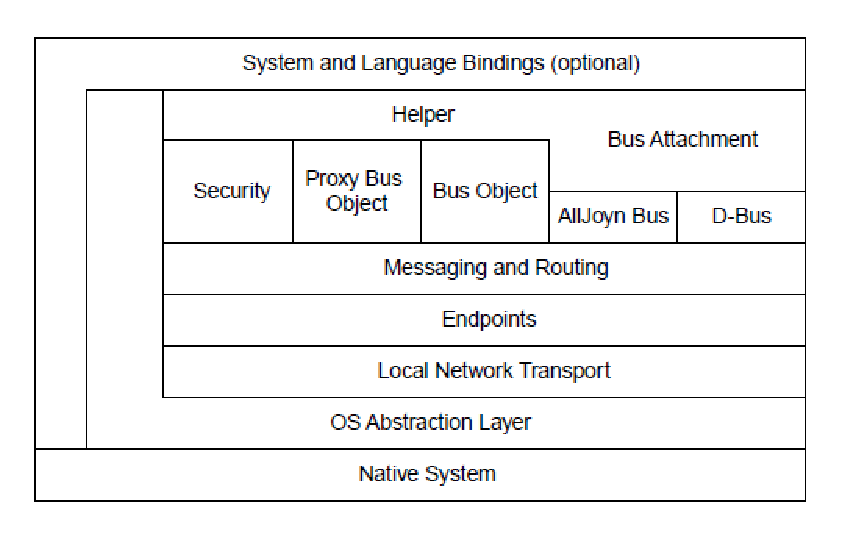
\includegraphics[height=3.5cm,width=6cm]{aj}}

\bb{Runtime architecture}
%\centerline{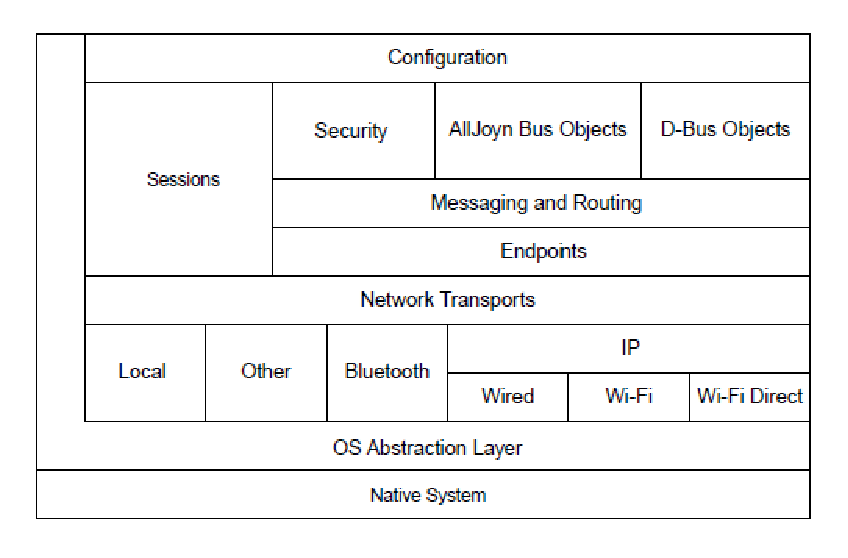
\includegraphics[height=3.5cm,width=6cm]{ajd}}


\end{frame}



\end{document}

%%  LocalWords:  RFID DSMS SQL CEP IFP Dataflow cep compsys softsys
